\subsection{Issue}
Ein \gls{Issue} entpricht im Sinne des Projektmanagement einem Arbeitspaket.
Ein solches \gls{Issue} hat eine Reihe von Eigenschaften oder Attributen.

\subsubsection{Title}
Der \gls{Title} ist die Kurzbeschreibung des \gls{Issue}. Dieser ist kurz und
prägnant gehalten und gibt eine grobe Angabe über dessen Inhalt.

\subsubsection{Comment}
Der \gls{Comment} zum Arbeitspaket. Hierbei gibt es zwei Arten von
\gls{Comment} die es zu unterscheiden gilt:

\begin{itemize}
	\item Initialier \gls{Comment}
	\item Alle anderen \gls{Comment}
\end{itemize}

Der initiale \gls{Comment} stellt eine detaillierte Beschreibung des
\gls{Issue} dar. Alle anderen \gls{Comment} bilden ein chronologisch
geordnetes Forum.

\subsubsection{Status \& Event}
Ein \gls{Issue} hat einen definierten zeitlichen Startpunkt, welcher durch
seinen Instanzierungszeitpunkt gegeben ist. Eine existenzielle
Terminierung ist hingegen nicht vorgesehen. Der Lebenszyklus eines
\gls{Issue} ist nicht abgeschlossen, hat also nur einen definierten Anfang
und kein Ende seiner Lebenszeit.

\begin{figure}[h!]
	\centering
	\begin{tikzpicture}[node distance=2.85cm,scale=0.75,transform shape]
		\node (start) [flowchart-block] {issue is created};
		\node (open) [flowchart-block, right of=start] {issue is open};
		\node (closed) [flowchart-block, right of=open] {issue is closed};
		\draw[->, thick, blue] (start) -- (open);
		\draw[->, thick, blue] (open) -- (closed);
		\draw[->, thick, blue] (closed) -- ++(2,0) -| ++(0,-2) -| (open);
		\draw[->, thick, dotted, red] (closed) ++(2,0) -- ++(2,0) node[anchor=west] {issue at end of life};
	\end{tikzpicture}
	\caption{Lebenszyklus eines issue}
\end{figure}

Während dieses Lebenszyklus können sich verschiedene \gls{Event} ereignen.
Diese sind zwischen den \gls{Comment} dargestellt und somit ebenfalls
chronologisch geordnet. Mögliche \gls{Event} sind dabei

\begin{itemize}
	\item close (\emph{Abschluss})
	\item reopen (\emph{Wiedereröffnung})
	\item assignment (\emph{Änderung der Zuständigkeit})
\end{itemize}

\subsubsection{Label}
Das \gls{Label} eines \gls{Issue} ist eine prägnante Markierung, welche mit
Text und Farbe eine Klassifizierung des \gls{Issue} darstellt. 

\subsubsection{Milestone}
Ein \gls{Issue} kann zu einem \gls{Milestone} gelinkt werden. Im Sinne des
Projektmanagement bedeutet dies, dass das \gls{Issue} dem angegebenen
\gls{Milestone} zugehörig ist. Somit ist der Abschluss des \gls{Issue}
eine zwingende Bedingung zur Erfüllen des \gls{Milestone}.

\subsubsection{Beispiel}

\begin{figure}[h!]
	\centering
	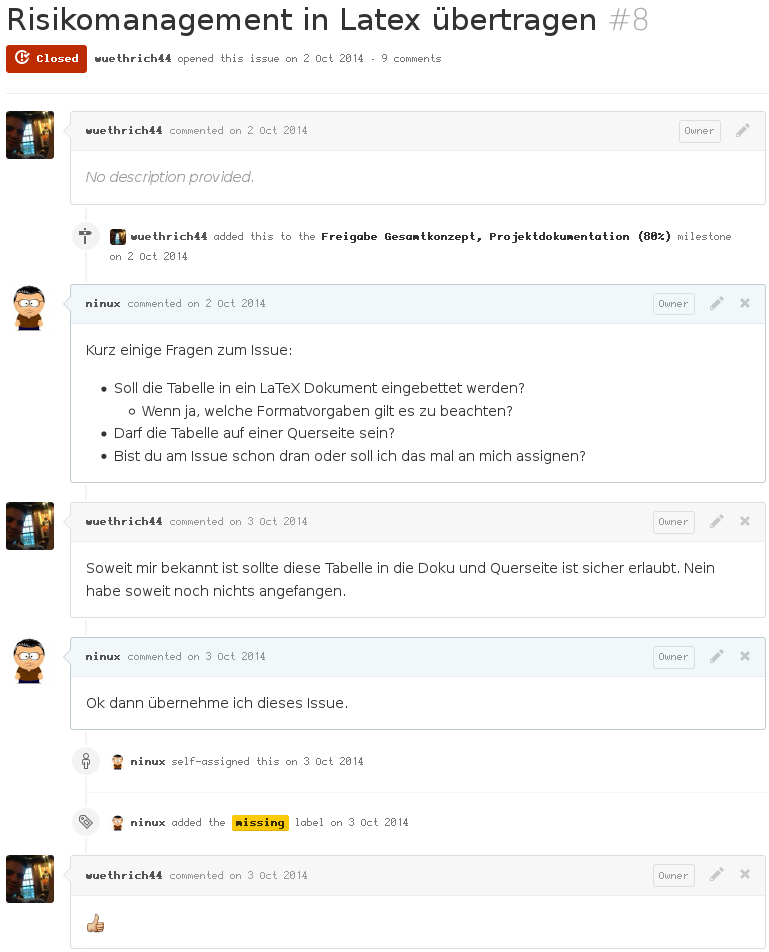
\includegraphics[width=0.75\textwidth]{../../fig/github/issue_comment.png}
	\caption{Auschschnitt aus der Historie eines Issues}
\end{figure}
